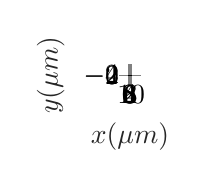
\begin{tikzpicture}
    \begin{axis}[%
width=0.9\figW,
height=0.15\figH,
at={(0\figW,0\figH)},
scale only axis,
axis on top,
xmin=0,
xmax=10,
xlabel style={font=\color{white!15!black}},
xlabel={$\text{x (}\mu\text{m)}$},
ymin=-2.5,
ymax=2.5,
ylabel style={font=\color{white!15!black}},
ylabel={$\text{y (}\mu\text{m)}$},
axis background/.style={fill=white},
]
\filldraw[fill=blue!40!white, draw=black] (0,1.95) rectangle (60,3.05);
\filldraw[fill=blue!10!white, draw=black, opacity=1] (5.2,2.5) rectangle (24.2,3.05);
\filldraw[fill=blue!10!white, draw=black, opacity=1] (35.8,2.5) rectangle (54.8,3.05);
\draw[draw=green, line width=1mm] (1,0.2) -- (1,4.8);
\draw[line width=0.8mm, draw=green, ->] (1.2,4) -- (5,4);
\draw[line width=0.8mm, draw=green, ->] (1.2,1) -- (5,1);
\end{axis}
\end{tikzpicture}